\textbf{Tercer parcial}
\begin{itemize}
%%Teoría flujo interno (mod 7)
 \item Explicar la vinculación entre las pérdidas de carga y los caudales en los casos en donde dos cañerías trabajan en paralelo.


%%Teoría máquinas hidráulicas (mod 8)
 \item ¿Cuál es la principal función de una bomba hidráulica?¿De qué parámetros de diseño depende su curva característica?
 \item ¿Cual es la principal función de una turbina hidráulica? ¿Qué es y para qué sirve el número específico de revoluciones?
 \item ¿Qué es y cómo se interpreta el punto de trabajo de una bomba en un sistema de cañerías?

%%Teoría Intro CFD (mod 9)




%%---------------------------------------------------------------------------



%% Ejercicios bombas e instalaciones
 \item Para el circuito de la figura \ref{fig:circuito} se dispone de una bomba centrífuga con un conjunto de 4 impulsores, tal como se  muestra en la curva correspondiente de la figura \ref{fig:bomba}. Completar los siguientes items:
 \begin{enumerate}
  \item Calcular las pérdidas energéticas y trazar las líneas de energía y  gradiente hidráulico.
  \item Seleccionar, mediante la figura \ref{fig:bomba},
  el impulsor que se adecue a las demandas del sistema. En caso de ser necesario, agregar los
  accesorios que permitan alcanzar las condiciones de servicio.
  \item Calcular el valor máximo de la distancia $L_asp$ (tramo 1-2 del circuito en figura \ref{fig:circuito})  en función del ANPA requerido por la bomba (esquema figura \ref{fig:ANPA}).
  \item Calcular la potencia total consumida por el equipo.
 \end{enumerate}

 \textbf{Despreciar las pérdidas localizadas.}. Fluido: agua (15 $\textordmasculine$C).
   
 Considerar el nivel de la cañería 1 coincidente con el piso (0 metros).

\begin{table}[!h]
  \centering
  \begin{tabular}{|l|c|c|p{2cm}|l|c|c|}
    \cline{1-3} \cline{5-7}
    \multicolumn{3}{|c|}{\textit{Datos}} && \multicolumn{3}{|c|}{\textit{Datos}} \\
    \cline{1-3} \cline{5-7}
    $\gamma$ & 1000 & $kg/m^3$ && $\nu$ & $10^{-6}$& $m^2/s$ \\
    \cline{1-3} \cline{5-7} 
    $p_{atm}$ & 10 & m.c.a. &&  $p_{vap}$ & 0.0176& bar \\ 
    \cline{1-3} \cline{5-7}
    $L_{asp}$ & 6 & m && $Z_{asp}$ & -2 & m \\
    \cline{1-3} \cline{5-7} 
    $L_1$ & 20 & m && $D_1$ & 0.15 & m \\ 
    \cline{1-3} \cline{5-7} 
    $L_2$ & 10 & m && $D_2$ & 0.04 & m \\ 
    \cline{1-3} \cline{5-7} 
    $L_3$ & 15 & m && $D_3$ & 0.05 & m \\ 
    \cline{1-3} \cline{5-7}
    $Z_A$ & 8 & m && $\mathbf{Q_A}$ & 40 & $m^3/h$ \\ 
    \cline{1-3} \cline{5-7}
    $Z_B$ & 8 & m && $\mathbf{Q_B}$ & 60 & $m^3/h$ \\ 
    \cline{1-3} \cline{5-7}
    $f$ & 0.022 &  && \multicolumn{2}{c|}{ANPA$_{req}$} & fig \ref{fig:ANPA}\\ 
    \cline{1-3} \cline{5-7} 
  \end{tabular}  
  \caption{Datos del problema 3}
  \label{tab:circuito}
  \end{table}

\begin{figure}[hb]
\centering
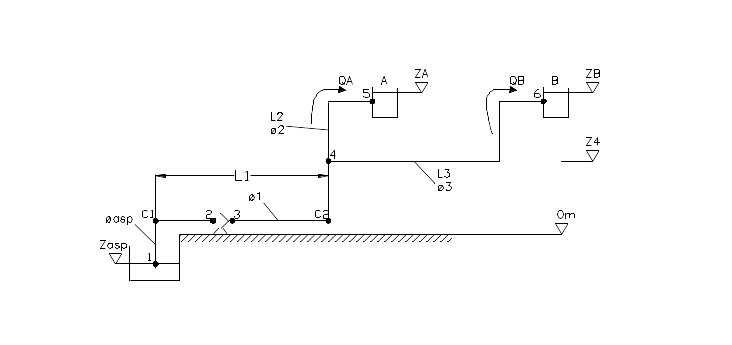
\includegraphics[width=0.8\textwidth]{circuitoGeneral.png}
\caption{Esquema del circuito}
\label{fig:circuito_gen}
\end{figure}


\begin{figure}[hb]
\centering
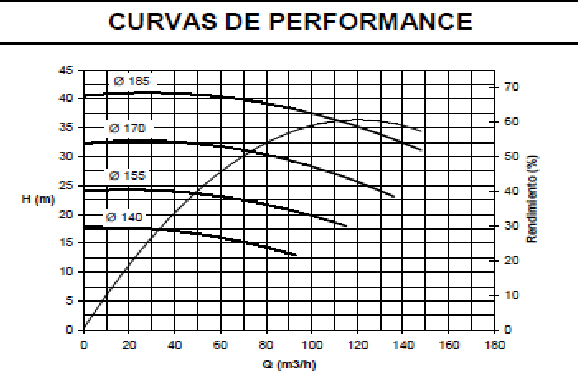
\includegraphics[width=\textwidth]{bomba.png}
\caption{Curvas características de la bomba disponible}
\label{fig:bomba}
\end{figure}

\begin{figure}[hb]
\centering
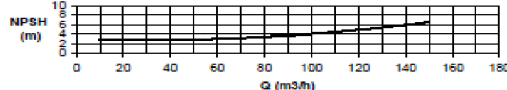
\includegraphics[width=\textwidth]{ANPA.png}
\caption{ANPA requerido por la bomba}
\label{fig:ANPA}
\end{figure}

%% 
 \item En el sistema de la figura (\ref{fig:circuito}) se deben cumplir las condiciones indicadas. Se dispone de dos bombas centrífugas idénticas, una instalada en el sistema y otra disponible para su uso en caso de ser necesario. Las características de las bombas  se detallan en la tabla.
 \begin{enumerate}
  \item Verificar si la bomba instalada cumple con las condiciones de servicio. En caso de no ser así, proponer soluciones.
  \item Calcular, de ser necesario, la pérdida de carga que debería generar una válvula para garantizar la distribución de caudales requerida por diseño.
%   \item Calcular la potencia que debe suministrar el motor a la bomba ($\eta_{mec}=0.92$)
 \end{enumerate}
 Considerar a su vez los siguientes datos:
 \begin{itemize}
  \item La velocidad de operación de la bomba es $n=1500RPM$.
  \item El fluido impulsado es agua ($\gamma = 1000 kgf/m^3$ y $\nu = 1 \times 10^{-6}m/s^2$).
  \item Las pérdidas locales son despreciables.
  \item El factor de Darcy de todas las cañerías puede aproximarse como $f=0.02$.
  \end{itemize}
  \vspace{-1cm}
\begin{figure}[!!!ht]
  \centering
   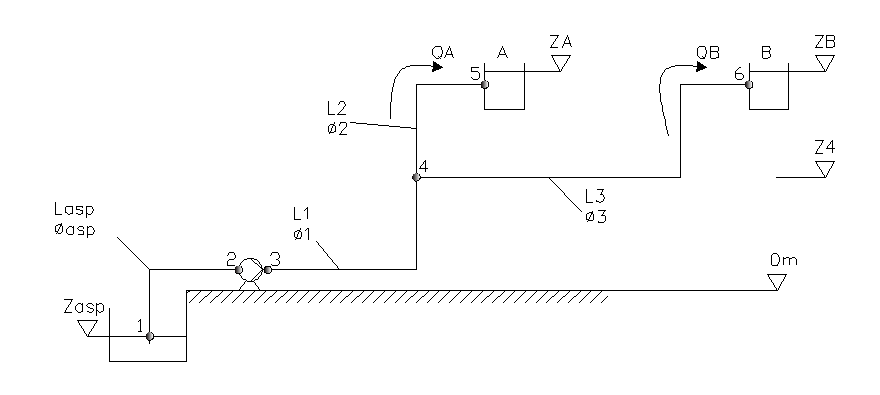
\includegraphics[width=14cm]{circuito.png}
  \caption{Esquema del circuito indicado}
  \label{fig:circuito}
  \end{figure}

  \begin{table}[!h]
  \centering
  \begin{tabular}{|l|c|c|c|c|r|}
    \hline 
    {\bf Q} & 100 & 150 & 350 & 500 & [$l/s$] \\ 
    \hline 
    {\bf H} & 98 & 95 & 93 & 89 & [$m$] \\ 
    \hline 
    $ANPA_{req}$ & 1.3 & 2.2 & 2.6 & 2.9 & [$m$] \\ 
    \hline 
  \end{tabular}  
  \caption{Propiedades de las bombas disponibles}
  \label{tab:bomba}
  \end{table}

\end{itemize}